%-------------------------------------------------------------------------------
%                            BAB III
%               		METODOLOGI PENELITIAN
%-------------------------------------------------------------------------------
\fancyhf{}
\fancyfoot[C]{\thepage}
\chapter{METODOLOGI PENELITIAN}

\section{\uppercase{WAKTU DAN LOKASI PENELITIAN}}
\setlength\parindent{30pt} Penelitian ini dilaksanakan di lantai 1 dan 3 di Gedung A FMIPA Universitas Syiah Kuala (USK). Waktu yang dibutuhkan untuk penelitian ini adalah 5 bulan terhitung dari bulan May 2021 hingga Oktober 2021.

\section{\uppercase{ALAT DAN BAHAN}}
Alat dan bahan yang digunakan pada penelitian ini meliputi perangkat keras, perangkat lunak dan bahan yang mendukung pada penelitian ini adalah data \textit{Received Signal Strength Indicator} (RSSI) dari hasil survei di lokasi penelitian. Adapun perangkat lunak yang digunakan adalah:
\begin{itemize}
	\itemsep0em
	\item OS Windows 10.
	\item Google Chrome.
	\item Visual Studio Code 1.59.1
	\item React Native
	\item MongoDB Compass 1.28.1
	\item Figma
	\item Postman 8.12.0
\end{itemize}

\par Sedangkan komponen perangkat keras yang digunakan meliputi 1 unit Laptop Acer dengan RAM 3GB, Intel® Core™ i3-3230M CPU @2.60Ghz (4 CPUs), ~2.6 GHz Processor, \textit{Harddisk} 500GB, \textit{Solid State Drive} (SSD) 120GB, memiliki Sistem Operasi Windows 64-bit, 20 unit \textit{KBeacon}, serta smartphone Samsung A30.

\section{\uppercase{METODE PENELITIAN}}
Metode penelitian yang dilakukan terdiri dari beberapa tahapan. Skema dari alur tahapan tersebut dapat dilihat pada Gambar \ref{metpen}.
\begin{figure}[H]
	\centering
	{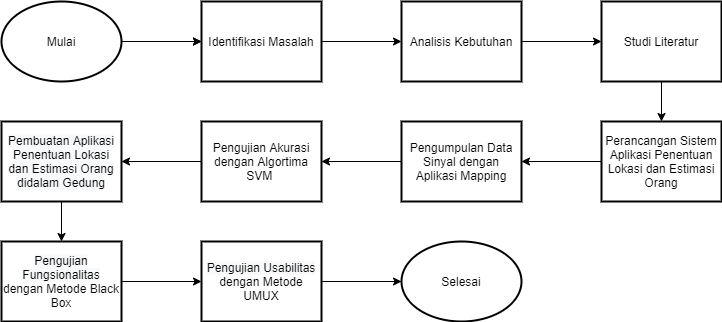
\includegraphics [width = 14cm, height= 6cm]{gambar/metodepenelitian.drawio }}
	\caption{Diagram Alir Penelitian}
	\label{metpen}
\end{figure}

\fancyhf{}
\fancyfoot[R]{\thepage}

\subsection{Identifikasi Masalah}
Tahapan ini adalah proses mengidentifikasi masalah sehingga aplikasi ini perlu dibuat. Adapun masalah yang diidentifikasikan adalah sebagai berikut:
\begin{enumerate}[1.]
	\itemsep0em
	\item Global Positioning System (GPS) belum bisa berfungsi jika digunakan dalam gedung.
	\item Pengguna buta arah perlunya petunjuk arah di dalam gedung
	      \citep{Keluza2017}.
	\item Perlunya data estimasi orang dalam gedung untuk pencegahan Covid-19
	\item Aplikasi untuk \textit{mapping} menyimpan data di local device sehingga tidak dapat dilakukan dengan banyak device sekaligus.
	\item Belum tersedia Aplikasi Penentuan Lokasi dan Estimasi Orang dalam Gedung .
\end{enumerate}

%%%%%%%%%%%%%%%%%%%%%%%%%%%%%%%%%%%%%%%%%%%
\subsection{Analisis Kebutuhan}
Pada tahapan ini, analisa kebutuhan bersumber dari masalah yang telah diidentifikasi pada tahap sebelumnya sehingga perancangan aplikasi dibangun sesuai kebutuhan. Adapun kebutuhan dari sistem yang dibangun adalah sebagai berikut:

\par \textbf{Kebutuhan Fungsional} Kebutuhan fungsional adalah fungsionalitas sistem itu sendiri. Adapun kebutuhan fungsional dari identifikasi masalah yang telah dilakukan adalah sebagai berikut:

\begin{itemize}
	\item Melakukan proses penentuan lokasi pengguna di dalam gedung FMIPA USK berbasis Crowdsourcing Indoor Localization System.

	\item Menampilkan prediksi lokasi pengguna saat berada di dalam gedung FMIPA USK.

	\item Menampilkan data estimasi orang di dalam gedung FMIPA USK.

\end{itemize}

\par \textbf{Kebutuhan Non-Fungsional} Kebutuhan non-fungsional memastikan batasan eksternal yang harus dipenuhi oleh sistem. Batasan-batasan tersebut antara lain:
\begin{itemize}
	\item System hanya dapat mendeteksi lokasi pengguna di dalam gedung yang telah dipetakan

	\item Dapat melakukan proses penentuan lokasi apabila bluetooth pada perangkat hidup dan terkoneksi dengan internet.

	\item Dapat mendata estimasi orang di dalam gedung.

\end{itemize}



%%%%%%%%%%%%%%%%%%%%%%%%%%%%%%%%%%%%%%%%%
\subsection{Studi Literatur}
Pada proses studi literatur, peneliti mengumpulkan bahan referensi penelitian yang bersumber dari jurnal-jurnal nasional dan internasional yang terkait penelitian ini dan situs \textit{website} serta buku-buku referensi untuk penelitian ini. Studi literatur dikembangkan untuk menyempurnakan penelitian sebelumnya.

\subsection{Perancangan Sistem}
Pada tahap ini, peneliti merancang alur kerja  sistem sehingga bisa memastikan sistem yang dirancang dapat digunakan sesuai kebutuhan pengguna. Alur kerja sistem dijelaskan menggunakan diagram alir yang dapat dilihat dari gambar berikut ini.
\ref{alur-kerja-sistem}.

\begin{figure}[H]
	\centering
	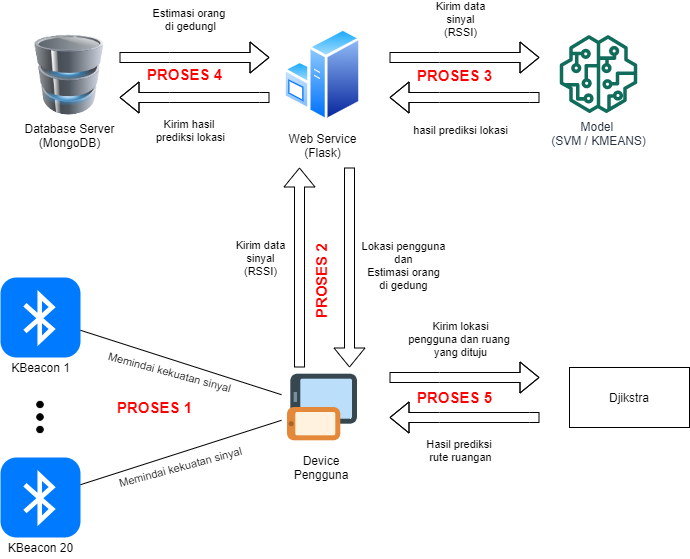
\includegraphics[width=10cm, height=8cm]{gambar/perancangansistem.png}
	\caption{Alur Kerja Sistem.}
	\label{alur-kerja-sistem}
\end{figure}

\subsection{Pembuatan Sistem}
Metode yang digunakan pada sistem ini adalah metode \textit{Scrum}. Metode \textit{Scrum} merupakan metodologi yang termasuk dalam agile software development. \textit{Scrum} dinilai dapat menghasilkan kualitas perangkat lunak yang baik sesuai dengan keinginan pengguna, dapat digunakan dalam proyek besar maupun kecil, dan mudah untuk mengadopsi perubahan.Sistem ini memiliki empat aplikasi yang terdiri dari tiga aplikasi utama dan satu aplikasi pendukung. yaitu:
\begin{enumerate}
	\item Aplikasi Penentuan Lokasi dan Estimasi Jumlah Orang
	      \newline Aplikasi ini merupakan aplikasi utama yang berfungsi untuk melakukan proses penentuan lokasi dan estimasi jumlah orang yang berada di dalam gedung A Fakultas Matematika dan Ilmu Pengetahuan Alam USK. Aplikasi ini dibangun menggunakan framework \textit{React native}

	\item Aplikasi \textit{Web Service Flask} Untuk Menjalankan Model \textit{Support Vector Machine} (SVM)
	      \newline Aplikasi \textit{Web Service Flask} merupakan aplikasi utama, yang mana aplikasi \textit{Web Service Flask} ini akan menjalankan model yang telah dihasilkan oleh kode bahasa \textit{python}.

	\item Aplikasi \textit{Mapping}
	      \newline Aplikasi ini merupakan aplikasi pendukung yang berfungsi untuk melakukan pengumpulan data. Data yang dikumpulkan berupa data kekuatan sinyal RSSI berdasarkan lokasi dimana data tersebut diambil. Setelah pengumpulan data selesai dilakukan, data tersebut akan di kirim ke \textit{Web Service GraphQL} dan kemudian akan di simpan ke \textit{Database MongoDB}.

	\item Aplikasi \textit{Web Service GraphQL} Untuk Menyimpan Data \textit{Mapping}
	      \newline Aplikasi \textit{Web Service GraphQL} merupakan aplikasi pendukung, yang mana aplikasi \textit{Web Service GraphQL} ini akan menyimpan data \textit{mapping} RSSI yang dikirimkan oleh \textit{device} peneliti.

\end{enumerate}

\subsection{Pengembangan Aplikasi Mapping}
\par Untuk memperoleh dataset untuk penelitian ini, maka diperlukan aplikasi \textit{mapping} untuk menangkap sinyal \text{bluetooth} dari alat \textit{Beacon}. Nilai RSSI yang diperoleh dari 20 \textit{Beacon} yang dipasang dari setiap sudut ruangan akan disimpan dalam database mongoDB. Pada penelitian sebelumnya, aplikasi \textit{mapping} menyimpan data di local server sehingga  tidak efektif jika digunakan oleh banyak server. Oleh karena itu, penulis merancang \textit{Web Service} agar data yang disimpan saat penelitian atau \textit{mapping} akan disimpan di database \textit{mongoDB}. Adapun fitur yang tersedia pada aplikasi \textit{mapping} ini adalah:

\begin {itemize}
\itemsep0em
\item Pemindaian Kekuatan Sinyal \newline
Aplikasi ini akan melakukan pemindaian kekuatan sinyal yang ditangkap dari setiap \textit{beacon} yang ditempel di setiap sudut ruangan, sehingga bisa menampilkan data RSSI, label, \textit{Mac Address}, nama \textit{beacon} yang ditandai tersebut.

\item Menyimpan Data Kekuatan Sinyal \newline
Ketika selesai melakukan \textit{mapping}, data kekuatan sinyal disimpan ke database \textit{mongoDB} yang berada di server. Data tersebut akan digunakan pada tahap penelitian selanjutnya.

\end{itemize}

%%%%%%%%%%%%%%%%%%%%%%%%%%%%%%%%%%%%%%%%%%%%%%%%%%%%%%%%%%%%%%%%%%%%%%%%%%%%%%%%%%%%%%%%%%%%%%%%%%%%%%%%%%%%%%%%%%
\subsection{Pengumpulan Data}
\begin{enumerate}[a.]
	\itemsep0em
	\item Pembuatan Denah Lokasi Penelitian
	      \\
	      Pembuatan Denah Lokasi Penelitian didasarkan pada rancangan gedung FMIPA USK. Denah ini dapat digunakan untuk menentukan posisi \textit{reference point} untuk proses pemetaan nantinya. Proses penentuan letak \textit{reference point} ini dilakukan dengan cara menghitung luas lokasi penelitian.
	      %%%%%%%%%%%%%%%%%%%%%%next%%%%%%%%%%%%%%%%%%%%%

	\item Pengukuran Jarak Lokasi Penelitian
	      \\
	      Pengukuran ini bertujuan untuk mengukur jarak dari denah lokasi penelitian yang telah dibuat. Hal ini agar bertujuan untuk membuat bobot pada algoritma \textit{Support Vector Machine} (SVM).

	\item Penentuan Letak \textit{Reference Point}
	      \\
	      Pada tahap ini, letak \textit{reference point} berada di gedung Blok A FMIPA USK, diantaranya adalah di lantai 1, tangga lantai 1 menuju lantai 2, tangga lantai 2 menuju lantai 3, koridor depan Laboratorium Jaringan Komputer, Laboratorium Database, dan Laboratorium Sistem Informasi Geografis.Penentuan letak \textit{reference point} ini dilakukan di setiap sudut ruangan kecuali di dalam ruangan laboratorium. Penentuan \textit{reference point} dilakukan secara urut dengan masing-masing jarak antara satu \textit{reference point} ke \textit{reference point} yang lain sejauh 2 ubin lantai atau 120 centimeter untuk meminimalisir \textit{position error}. \citep{Lee2019} \citep{Bahl2000}. Tujuan penentuan posisi \textit{reference point} ini bertujuan untuk menentukan lokasi pengumpulan data kekuatan sinyal yang dipancarkan setiap \textit{Beacon} di setiap sudut ruangan. Penentuan \textit{reference point} yang saling berdekatan mempengaruhi hasil tahap \textit{positioning}. Denah lokasi penelitian ini dapat dilihat pada Gambar \ref{gedungA}.

	      %\vspace{2cm}
	      \begin{figure}[H]
		      \centering
		      \subfloat[Denah Lantai 1]{{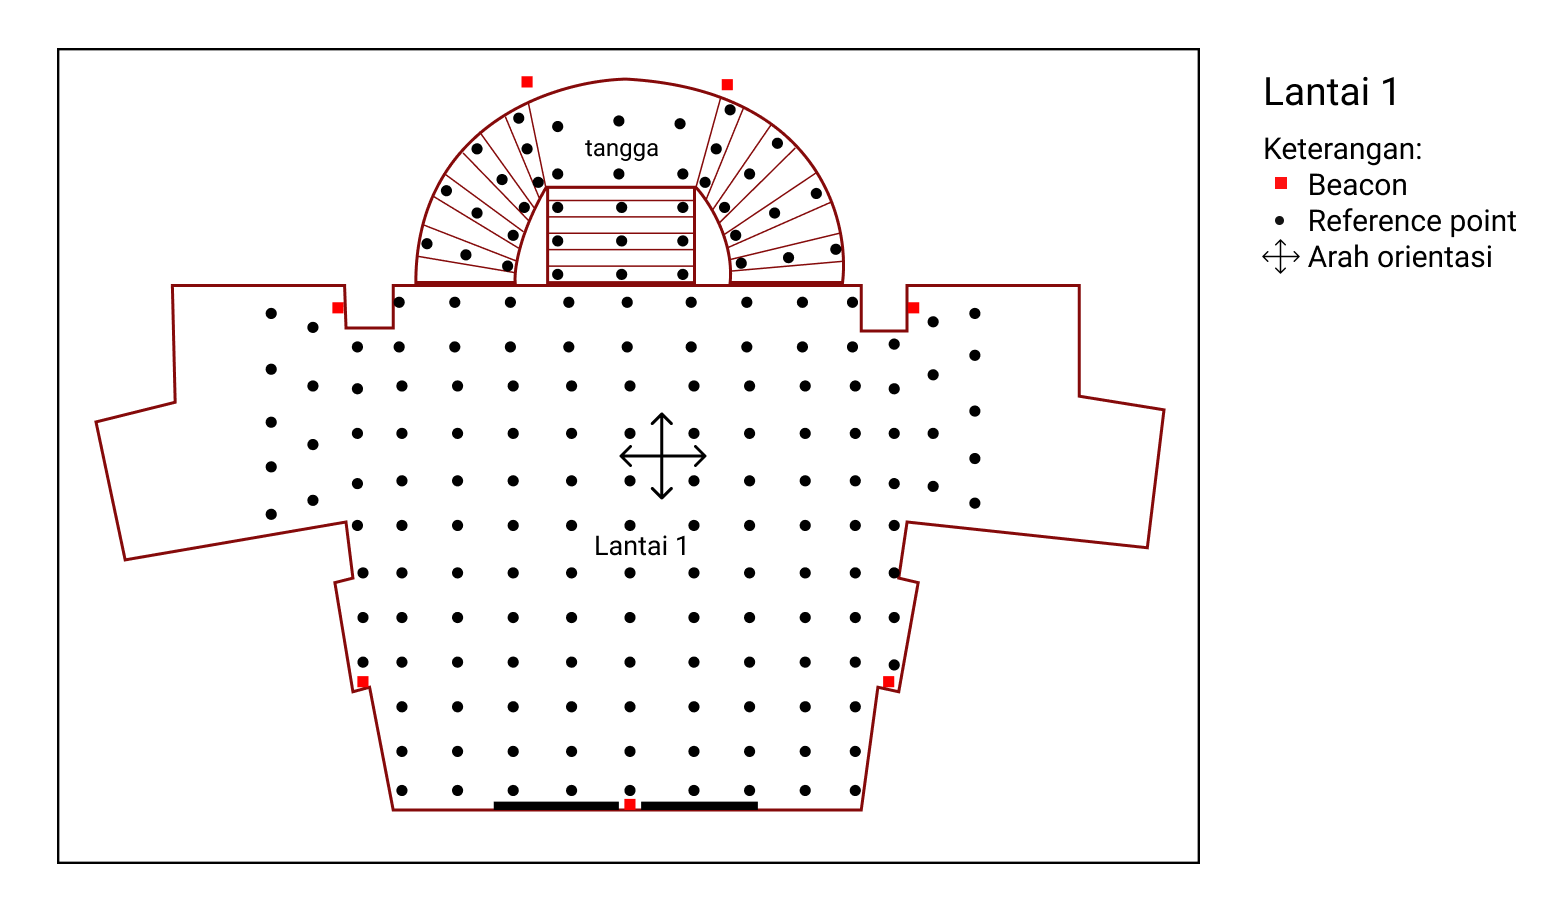
\includegraphics[width=13cm, height=7cm]{gambar/Lantai1} }}%
		      \qquad
		      \subfloat[Denah Lantai 2]{{\includegraphics[width=13cm, height=8cm]{gambar/lantai2} }}

		      \centering
		      \subfloat[Denah Lantai 3]{{\includegraphics[width=12cm, height=6cm]{gambar/lantai3} }}
		      \caption{Ilustrasi Denah Lokasi Letak \textit{Reference Point} Penelitian Gedung Blok A FMIPA}%
		      \label{gedungA}%
	      \end{figure}

	      \par Pada proses ini, masing-masing \textit{reference point} saat mengambil kekuatan sinyal akan menghadap 4 arah oriental yaitu depan, belakang, kiri dan kanan.Kekuatan sinyal pada lokasi tertentu memiliki nilai yang bervariasi hingga -5 dBm tergantung orientasi yang dihadapi pengguna \cite{Bahl2000}. Tiap arah orientasi, antena \textit{host} yang dimiliki oleh \textit{smartphone} memiliki konektivitas \textit{line-of-sight} (LoS) ke sebuah antena \textit{Beacon} selama orientasinya berlawanan. Arah orientasi dari tubuh pengguna juga dapat menimbulkan halangan dan kekuatan sinyal yang ditangkap juga berbeda. Oleh karena itu, perlu dilakukan pencatatan \textit{direction} (d), dengan menghadap ke depan, ke kanan, ke belakang dan ke kiri tergantung pada pengambilan kekuatan sinyal yang dilakukan \citep{christ1993}. Metode pengambilan kekuatan sinyal setiap \textit{Beacon} berdasarkan proses survei pemetaan \textit{reference point} disebut dengan metode \textit{Fingerprinting}. Metode \textit{Fingerprinting} dilakukan dengan mengumpulkan  data-data kekuatan sinyal tersebut ke dalam basis data \textit{mongoDB} untuk dijadikan sebagai data \textit{training} nantinya.

	      %%%%%%%%%%%%%%%%%%%%%%next%%%%%%%%%%%%%%%%%%%%%
	\item Pengumpulan Data \textit{Training}
	      \par
	      Basis data yang berisikan data \textit {training} yaitu data kekuatan sinyal dengan nilai RSSI yang didapatkan dari tiap \textit{beacon} dilakukan berdasarkan penentuan letak \textit{reference point} yang telah ditentukan pada tahap sebelumnya. Pengumpulan data \textit{training} dengan pemetaan metode \textit{Fingerprinting} ini menggunakan Aplikasi Mapping yang telah dibuat dengan fitur-fitur untuk dapat menangkap kekuatan sinyal dari \textit{Beacon}, kemudian informasi-informasi dari \textit{Beacon} tersebut seperti MAC Address, nilai RSSI, dan nama ruangan dimana kekuatan sinyal tersebut ditangkap dapat disimpan pada server. Ilustrasi penyimpanan data \textit{training} dengan metode \textit{Fingerprinting} untuk \textit{reference point} dapat dilihat pada Tabel \ref{fingerprinting}. Orientasi yang tercantum pada gambar tersebut hanya sebagai gambaran bahwa penyimpanan data terhadap suatu posisi diambil berdasarkan 4 arah orientasi.

	      \begin{landscape}
		      \begin{table}[H]
			      \caption{Ilustrasi Penyimpanan Data Training Metode \textit{Fingerprinting} pada \textit{Reference Point}}
			      \centering
			      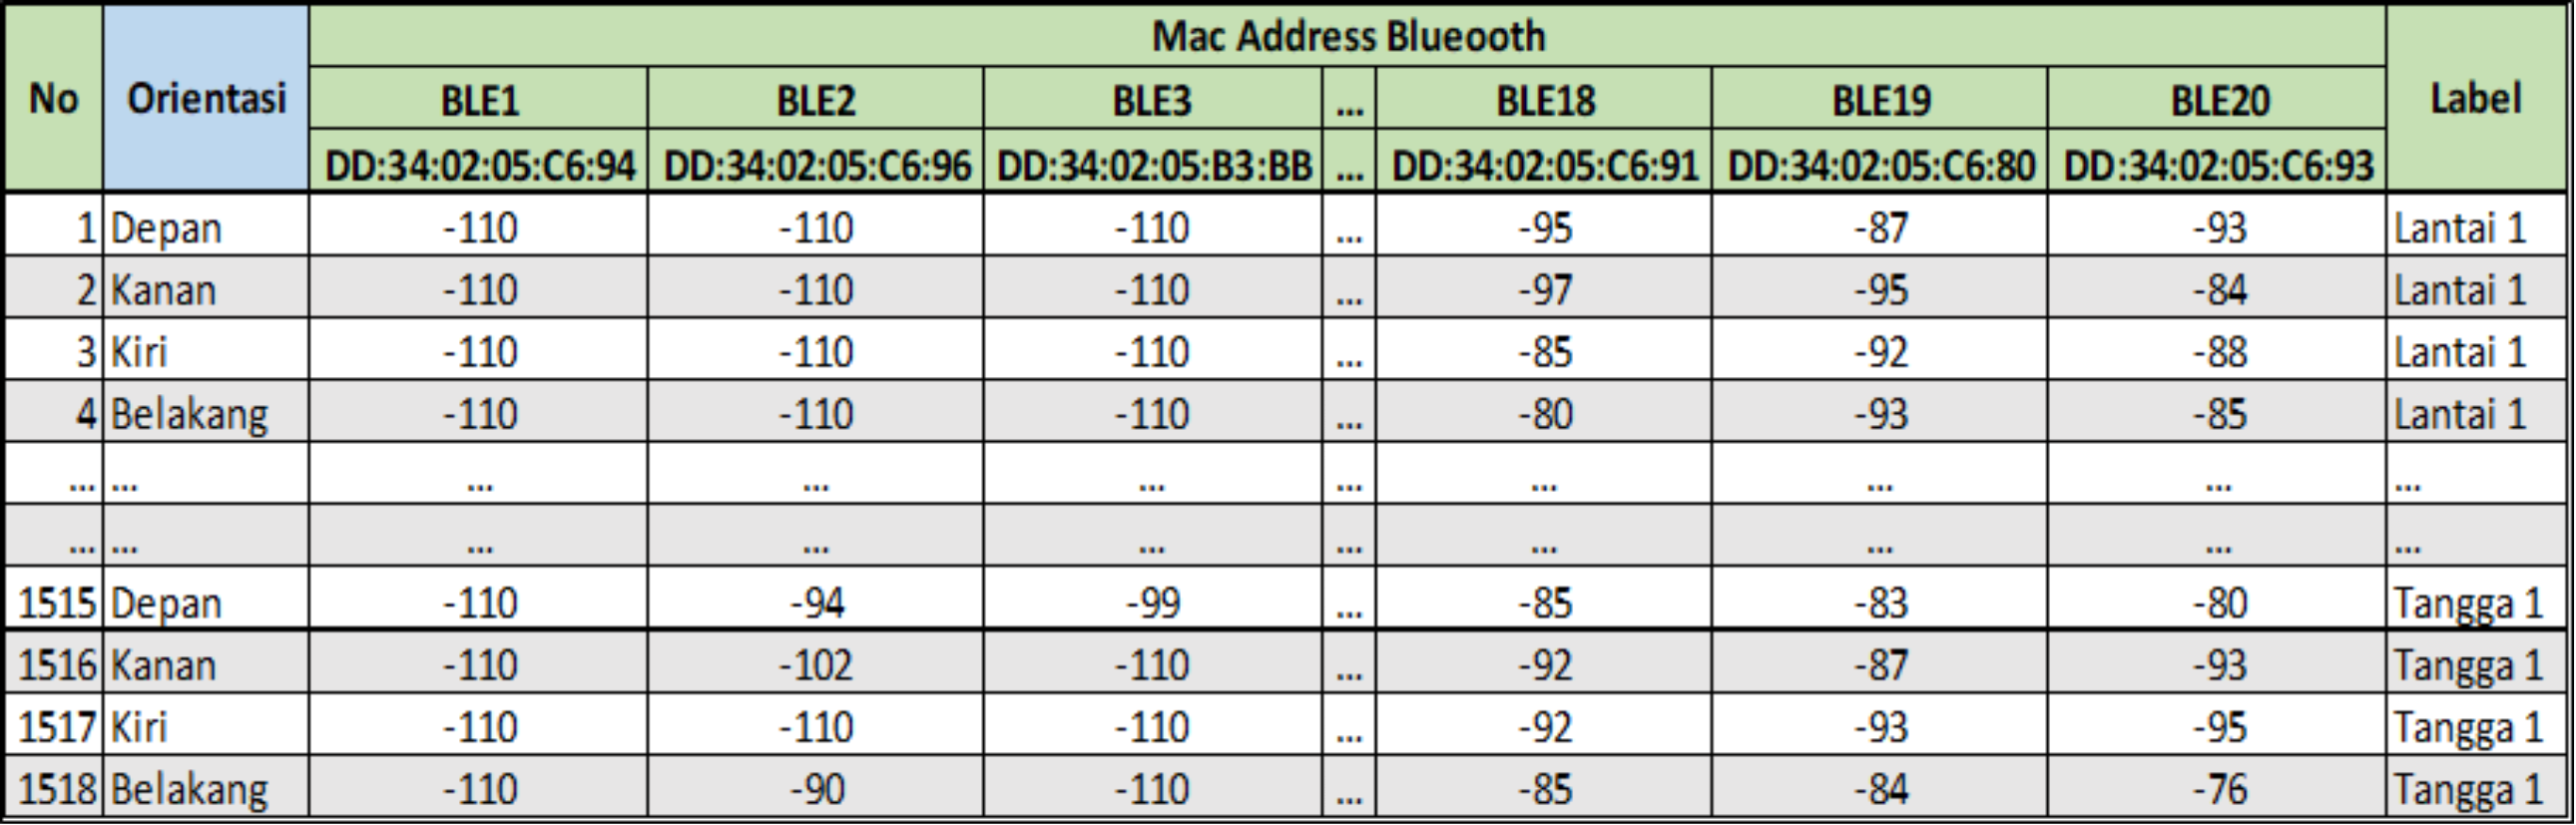
\includegraphics[width=25cm, height=7cm]{gambar/tes}
			      \label{fingerprinting}
		      \end{table}
	      \end{landscape}



	      \vspace{3cm}

	\item Pengumpulan Data Uji
	      \\
	      Pengumpulan data uji dilakukan setelah pengumpulan data \textit{training}. Data uji bertindak seolah-olah kelas label belum diketahui. Data uji tersebut akan dibandingkan dengan data \textit{training}, hasil tersebut akan diimplementasikan pada Aplikasi Penentuan Lokasi dan Estimasi Orang di dalam Gedung untuk memprediksi lokasi pengguna dengan metode klasifikasi \textit{Support Vector Machine} (SVM).

\end{enumerate}
%%%%%%%%%%%%%%%%%%%%%%%%%%%%%%%%%%%%%%%%%%%%%%%%%%%%%%%%%%%%%%%%%%%%%%%%%%%%%%%%%%%%%%%%%%%%%%%%%%%%%%%%%%%%%%%%%%%%%%%%%%%
%TESTING svm%
\subsection{Pengujian Akurasi dengan Metode Klasifikasi SVM}

\par Pengujian ini dilakukan dengan tujuan untuk mengetahui tingkat keberhasilan prediksi dengan menggunakan algoritma \textit{Support Vector Machine} (SVM) terhadap lokasi pengguna berdasarkan \textit{reference point} yang digunakan. Algoritma klasifikasi SVM pada penelitian ini dibuat dengan menggunakan kode python dengan tahapan sebagai berikut :

\begin{enumerate}[1.]
	\itemsep0em
	\item \textit{Import} library yang diperlukan
	      %   \begin{figure}[H]
	      %       \centering
	      %       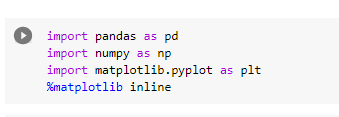
\includegraphics[width=14cm, height=3.5cm]{gambar/uji1}
	      %       \caption{\textit{Import} library yang diperlukan}
	      %       \label{uji1}
	      %   \end{figure}



	\item Memproses data atau membaca dataset dari hasil mapping
	      %   \begin{figure}[H]
	      %       \centering
	      %       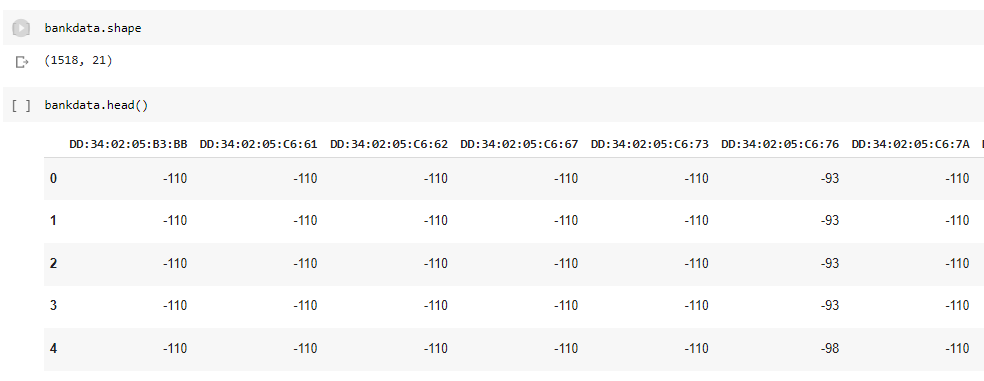
\includegraphics[width=14cm, height=6cm]{gambar/uji2}
	      %       \caption{Pemprosesan data atau membaca dataset dari hasil mapping}
	      %       \label{uji2}
	      %   \end{figure}

	\item Membagi data menjadi atribut dan label
	      %   \begin{figure}[H]
	      %       \centering
	      %       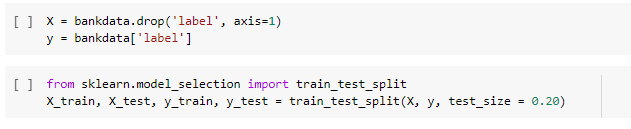
\includegraphics[width=14cm, height=4cm]{gambar/uji3}
	      %       \caption{Pembagian data menjadi atribut dan label}
	      %       \label{uji3}
	      %   \end{figure}

	\item Melatih Algoritma
	      %   \begin{figure}[H]
	      %       \centering
	      %       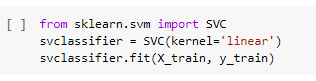
\includegraphics[width=13cm, height=4cm]{gambar/uji4}
	      %       \caption{Melatih Algoritme}
	      %       \label{uji4}
	      %   \end{figure}

	\item Menghasilkan model dan visualisasi hasil algoritma SVM.
	      \par Hasil tersebut adalah hasil akurasi dari klasifikasi algoritma SVM. Model dari algoritma SVM juga nantinya akan digunakan untuk memprediksi lokasi pengguna dalam penerapan aplikasi nantinya.

	\item Memprediksi
	      \par Proses ini akan memprediksi dengan memasukkan data \textit{testing} yang didapat dari proses pengambilan data uji menggunakan kode \textit{python}.
\end{enumerate}

\subsection{Pembuatan Model SVM}
Pada proses pembuatan model ini, dilakukan setelah proses pengujian akurasi dengan menggunakan algoritma klasifikasi \textit{Support Vector Machine} (SVM) dirasa sudah lebih akurat dengan dapat memprediksi semua klasifikasi yang diharapkan. Model dibuat dengan menggunakan bahasa kode python yang memanfaatkan library dari python yaitu \textit{pandas}, \textit{numpy}, dan \textit{matplotlib}. Setelah model berhasil dibuat maka model akan dimasukkan ke dalam \textit{web service flask}, dari \textit{web service flask} ini akan menghasilkan prediksi dari model dan akan dikirim ke aplikasi utama.


\subsection{Pembuatan Aplikasi Penentuan Lokasi dan Estimasi Orang dalam Gedung}
\begin{enumerate}


	\item Aplikasi Penentuan Lokasi dan Estimasi Jumlah Orang di dalam Gedung
	      \newline
	      Aplikasi yang dibangun menggunakan \textit{react native} ini adalah aplikasi berbasis Android yang berguna untuk mempermudah pengguna dan rekan tim penelitian untuk melakukan proses
	      pencarian lokasi dan estimasi jumlah orang yang berada di dalam gedung Blok A Fakultas Matematika dan Ilmu Pengetahuan Alam Universitas Syiah Kuala, yang dikembangkan dengan konsep \textit{Indoor Localization System} dan \textit{Crowdsourcing}. Aplikasi ini bekerja apabila perangkat smartphone sudah mendukung Bluetooth 4.0, dikarenakan aplikasi ini menangkap kekuatan sinyal atau nilai RSSI dari \textit{Beacon} yang terintegrasi BLE di dalamnya. Kekuatan sinyal yang ditangkap akan dilakukan perhitungan menggunakan metode klasifikasi \textit{Support Vector Machine} (SVM), output dari perhitungan tersebut adalah prediksi lokasi pengguna yang akan dikirim ke web services flask secara background process. Adapun fitur-fitur yang tersedia adalah sebagai berikut:.

	      \begin {itemize}
	      \itemsep0em
	\item Memprediksi Lokasi Pengguna saat berada di dalam gedung\newline

	\item Menampilkan Estimasi Jumlah Orang yang Berada di dalam Gedung Blok A Fakultas Matematika dan Ilmu Pengetahuan Alam Universitas Syiah Kuala

	      \end{itemize}
\end{enumerate}
%%%%%%%%%%%%%%%%%%%%%%%%%%%%%%%%%%%%%%%%%%%%%%%%%%%%%%%%%%%%%%%%%%%%%%%%%%%%%%%%%%%%%%%%%%%%%%%%%%%%%%%%%%%%%%%%%%%%%%%%%%%%%%%
\subsection{Pengujian Fungsionalitas dengan Metode Black Box}
\par Pengujian \textit{Black Box} berfokus pada spesifikasi fungsionalitas dari sistem yang telah dibuat dengan mengeksekusi dan menjalankan sistem tersebut apakah sesuai dengan alur bisnis yang diinginkan. Pengujian ini melihat fungsi yang tidak sesuai pada sistem, kesalahan-kesalahan sistem dalam mengerjakan suatu perintah, dan kesalahan-kesalahan pada struktur data dan akses basis data.

\subsection{Pengujian \textit{Usabilitas} dengan Metode UMUX}
\par \textit{Usability Testing} dilakukan untuk melihat dan mengevaluasi suatu produk atau jasa yang dihasilkan dengan cara menguji kepada calon pengguna dengan menggunakan metode UMUX. UMUX terdiri dari 4 pertanyaan dengan menggunakan skala likert 1-7.
\par Skala likert adalah sebuah metode skala yang bersifat bipolar yang akan mengukur tanggapan positif dan negatif terhadap sebuah pertanyaan.
Berikut daftar pertanyaan-pertanyaan metode UMUX dapat dilihat pada Tabel \ref{tabel-pertanyaan-umux}.
%TABEL PERTANYAAN SUS%
\begin{table}[H]
	\center
	\caption{Daftar Pertanyaan Metode UMUX \citep{Finstad2010}}
	\label{tabel-pertanyaan-umux}
	\begin{tabular}{|l|l|l|}
		\hline
		\rowcolor[HTML]{656565}
		{\color[HTML]{343434} No.} & Pertanyaan                                                                                                                 & Skor \\ \hline
		1                          & Aplikasi ini sesuai dengan kebutuhan saya                                                                                  & 1-7  \\
		\hline
		2                          & Saya memiliki pengalaman buruk dalam menggunakan aplikasi ini                                                              & 1-7  \\
		\hline
		3                          & Aplikasi ini mudah digunakan                                                                                               & 1-7  \\
		\hline
		4                          & \begin{tabular}[c]{@{}l@{}}Saya harus mengabiskan banyak waktu \\ untuk menggunakan aplikasi ini dengan benar\end{tabular} & 1-7  \\ \hline
	\end{tabular}
\end{table}

% \subsection{Pengujian Usability dengan Metode SUS}
% \par Salah satu prinsip utama yang dijadikan sebagai tolak ukur keberhasilan dari pengembangan perangkat lunak adalah nilai pengujian itu sendiri. \textit{Usability Testing} dilakukan untuk melihat dan mengevaluasi sebuah produk atau jasa dengan cara menguji kepada calon pengguna dengan menggunakan metode SUS. SUS terdiri dari 10 pertanyaan dengan menggunakan skala likert 1-5. Berikut daftar pertanyaan-pertanyaan metode SUS dapat dilihat pada Tabel \ref{tabel-pertanyaan-sus}.
% %TABEL PERTANYAAN SUS%
% \begin{table}[H]
% 	\center
% 	\caption{Daftar Pertanyaan Metode SUS \citep{Sharfina2016}}
% 	\label{tabel-pertanyaan-sus}
% 	\begin{tabular}{|c|l|l}
% 		\cline{1-2}
% 		\textbf{\begin{tabular}[c]{@{}c@{}}Kode \\ Pertanyaan\end{tabular}} & \multicolumn{1}{c|}{\textbf{Daftar Pertanyaan}}                                                                               & \\ \cline{1-2}
% 		$R1$                                                                & Saya berpikir akan menggunakan sistem ini                                                                                     & \\ \cline{1-2}
% 		$R2$                                                                & Saya merasa sistem ini sulit untuk digunakan                                                                                  & \\ \cline{1-2}
% 		$R3$                                                                & Saya merasa sistem ini mudah digunakan                                                                                        & \\ \cline{1-2}
% 		$R4$                                                                & \begin{tabular}[c]{@{}l@{}}Saya akan membutuhkan bantuan orang lain \\ untuk menggunakan sistem ini\end{tabular}              & \\ \cline{1-2}
% 		$R5$                                                                & \begin{tabular}[c]{@{}l@{}}Saya merasa fitur-fitur pada sistem ini sudah \\ berjalan dengan sebagaimana mestinya\end{tabular} & \\ \cline{1-2}
% 		$R6$                                                                & \begin{tabular}[c]{@{}l@{}}Saya merasa banyak hal-hal yang tidak \\ konsisten (tidak serasi) pada sistem ini\end{tabular}     & \\ \cline{1-2}
% 		$R7$                                                                & \begin{tabular}[c]{@{}l@{}}Saya merasa orang lain dapat memahami cara\\ menggunakan aplikasi ini dengan cepat\end{tabular}    & \\ \cline{1-2}
% 		$R8$                                                                & Saya merasa aplikasi ini membingungkan                                                                                        & \\ \cline{1-2}
% 		$R9$                                                                & \begin{tabular}[c]{@{}l@{}}Saya merasa nyaman (tidak ada hambatan) \\ dalam menggunakan sistem ini\end{tabular}               & \\ \cline{1-2}
% 		$R10$                                                               & \begin{tabular}[c]{@{}l@{}}Saya perlu membiasakan diri terlebih dahulu \\ sebelum menggunakan aplikasi ini\end{tabular}       & \\ \cline{1-2}
% 	\end{tabular}
% \end{table}

% \par Rumus untuk menghitung skor akhir metode SUS \citep{Brooke1996}, dapat dilihat dari persamaan berikut.
% \begin{equation}
% 	skorSUS = (\sum_{9}^{i} (Ri - 1) + \sum_{10}^{j} (5 - Rj)) * 2,5
% \end{equation}
% \newline
% Keterangan:\newline
% $R$ = daftar pertanyaan pada metode SUS. \newline
% $i$ = angka ganjil 1, 3, 5, 7, dan 9. \newline
% $j$ = angka genap 2, 4, 6, 8, dan 10.
% \newline

% \par Tingkat nilai skala pengujian menentukan apakah sistem tersebut layak digunakan, bermanfaat, diterima oleh \textit{user} dan bertahan lama penggunaannya. Sebuah sistem dengan nilai pengujian yang tinggi membuat sistem tersebut menjadi populer dalam waktu yang lama dan penggunaannya yang luas, karena banyak individu akan merasakan manfaat dari kehadiran sistem tersebut. Sedangkan sistem dengan nilai pengujian yang rendah, seringkali diabaikan oleh pengguna walaupun dibuat berdasarkan kebutuhan dan menghasilkan sumber daya yang banyak. Berdasarkan dari skor akhir SUS tersebut, dapat diketahui bahwa seberapa tinggi tingkat \textit{usability} perancangan sistem yang dikembangkan. Tabel \ref{tabelsus} menunjukkan nilai interpretasi yang digunakan.

% \begin{table}[H]
% 	\center
% 	\caption{Interpretasi skor SUS \citep{Bangoor2009}.}
% 	\label{tabelsus}
% 	\begin{tabular}{|c|c|lll}
% 		\cline{1-2}
% 		\textbf{Skor SUS} & \textbf{Interprestasi} &  &  & \\ \cline{1-2}
% 		\textless{}50     & Tidak Dapat Diterima   &  &  & \\ \cline{1-2}
% 		50-70             & Marginal               &  &  & \\ \cline{1-2}
% 		\textgreater{}70  & Dapat Diterima         &  &  & \\ \cline{1-2}
% 	\end{tabular}
% \end{table}

%%%%%%%%%%%%%%%%%%%%%%%%%%%%%%%%%%%%%%%%%%%%%%%%%%%%%%%%%%%%%%%%%%%%%%%%%%%%%%%%%%%%%%%%%%%%%%%%%%%%%%%%%%%%%%%%
\subsection{Analisis Keakuratan}
Penelitian ini memiliki dua analisis keakuratan yaitu dalam penentuan lokasi pengguna dan estimasi jumlah orang saat berada di gedung A Fakultas Matematika dan Ilmu Pengetahuan Alam Universitas Syiah Kuala. Analisis keakuratannya adalah sebagai berikut:
\begin{enumerate}[1.]
	\item Melihat seberapa akurat prediksi lokasi pengguna dengan menggunakan algoritma \textit{Support Vector Machine} (SVM).
	\item Melihat seberapa akurat prediksi estimasi orang di dalam gedung dengan menggunakan metode \textit{crowdsourcing}.
\end{enumerate}
